\documentclass[a4paper]{article}
\usepackage[newfloat]{minted}
\usepackage{graphicx}
\usepackage{caption}
\usepackage{amsmath}
\usepackage{amsfonts}
\usepackage[a4paper,left=3cm,right=2cm,top=2.5cm,bottom=2.5cm]{geometry}
\usepackage[colorlinks=true, urlcolor=blue, pdfborder={0 0 0}]{hyperref}
\newenvironment{code}{\captionsetup{type=listing}}{}
\SetupFloatingEnvironment{listing}{name=Code}

\title{RL Homework 2}
\author{Ananth Mahadevan}
\begin{document}
\maketitle
\clearpage
\tableofcontents
\clearpage

\section{Question 1}
\textbf{Answer:} The agent in the given setup is the sailor and by extension the boat he controls.The actions available  to the agent are only the ability to choose to go left,right, up or down. The wind, the water, the rocks, the harbour and all other locations and entities are the environment in the setup. 
\section{Question 2}
Once we run value iteration for 100 iteration the value of the states are as seen in Figure~\ref{fig-sailor}.
\begin{figure}[ht!]
    \centering
    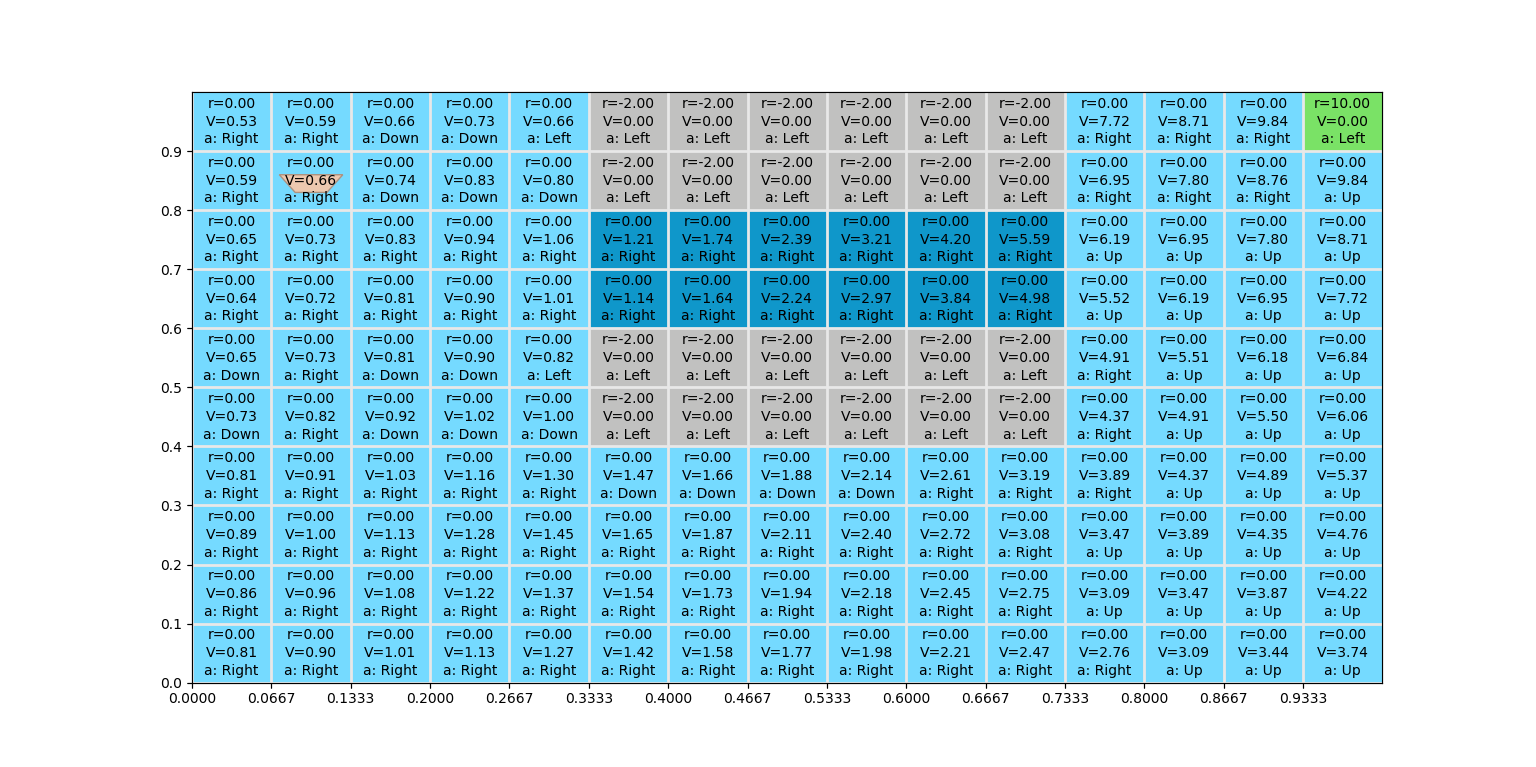
\includegraphics[width=\textwidth]{Sailor.png}
    \caption{Grid Details after Value Iteration and Policy Updation}
    \label{fig-sailor}
\end{figure}
This gives us the answer that the harbour and the rocks have value of $\mathbf{0}$. The reason is because as these states are the terminal states the expectation of possible future rewards when starting from these states is always 0, as the game always terminates, hence value iteration also converges on the value of theses states being 0.
\section{Question 3}
If we consider the optimal actions at every state from the starting state and assuming that the optimal action action is executed to reach the state, then we can trace the path on expectation that the sailor will take. This is shown as the red path in Figure~\ref{fig-sailor-path}
\begin{figure}[ht!]
    \centering
    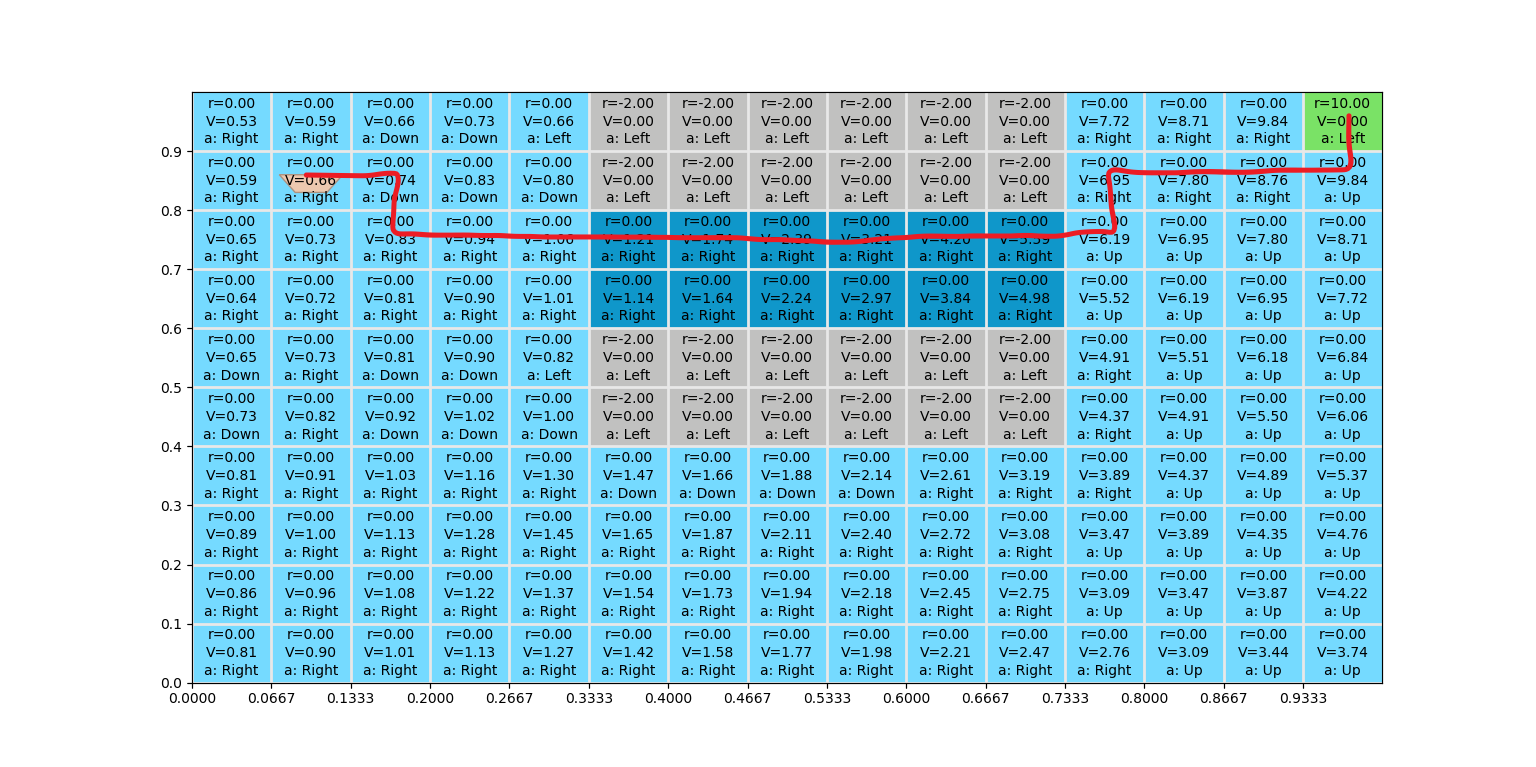
\includegraphics[width=\textwidth]{Sailor_path.png}
    \caption{Optimal Path of Sailor for standard setting}
    \label{fig-sailor-path}
\end{figure}
If we now change the reward for hitting a rock to $\mathbf{-10}$, then the sailor gets \textbf{\textit{paranoid}} about hitting rocks, hence chooses a different \textbf{safer} path based on the recomputed state values as seen in Figure~\ref{fig-paranoid-sailor-path}
\begin{figure}[ht!]
    \centering
    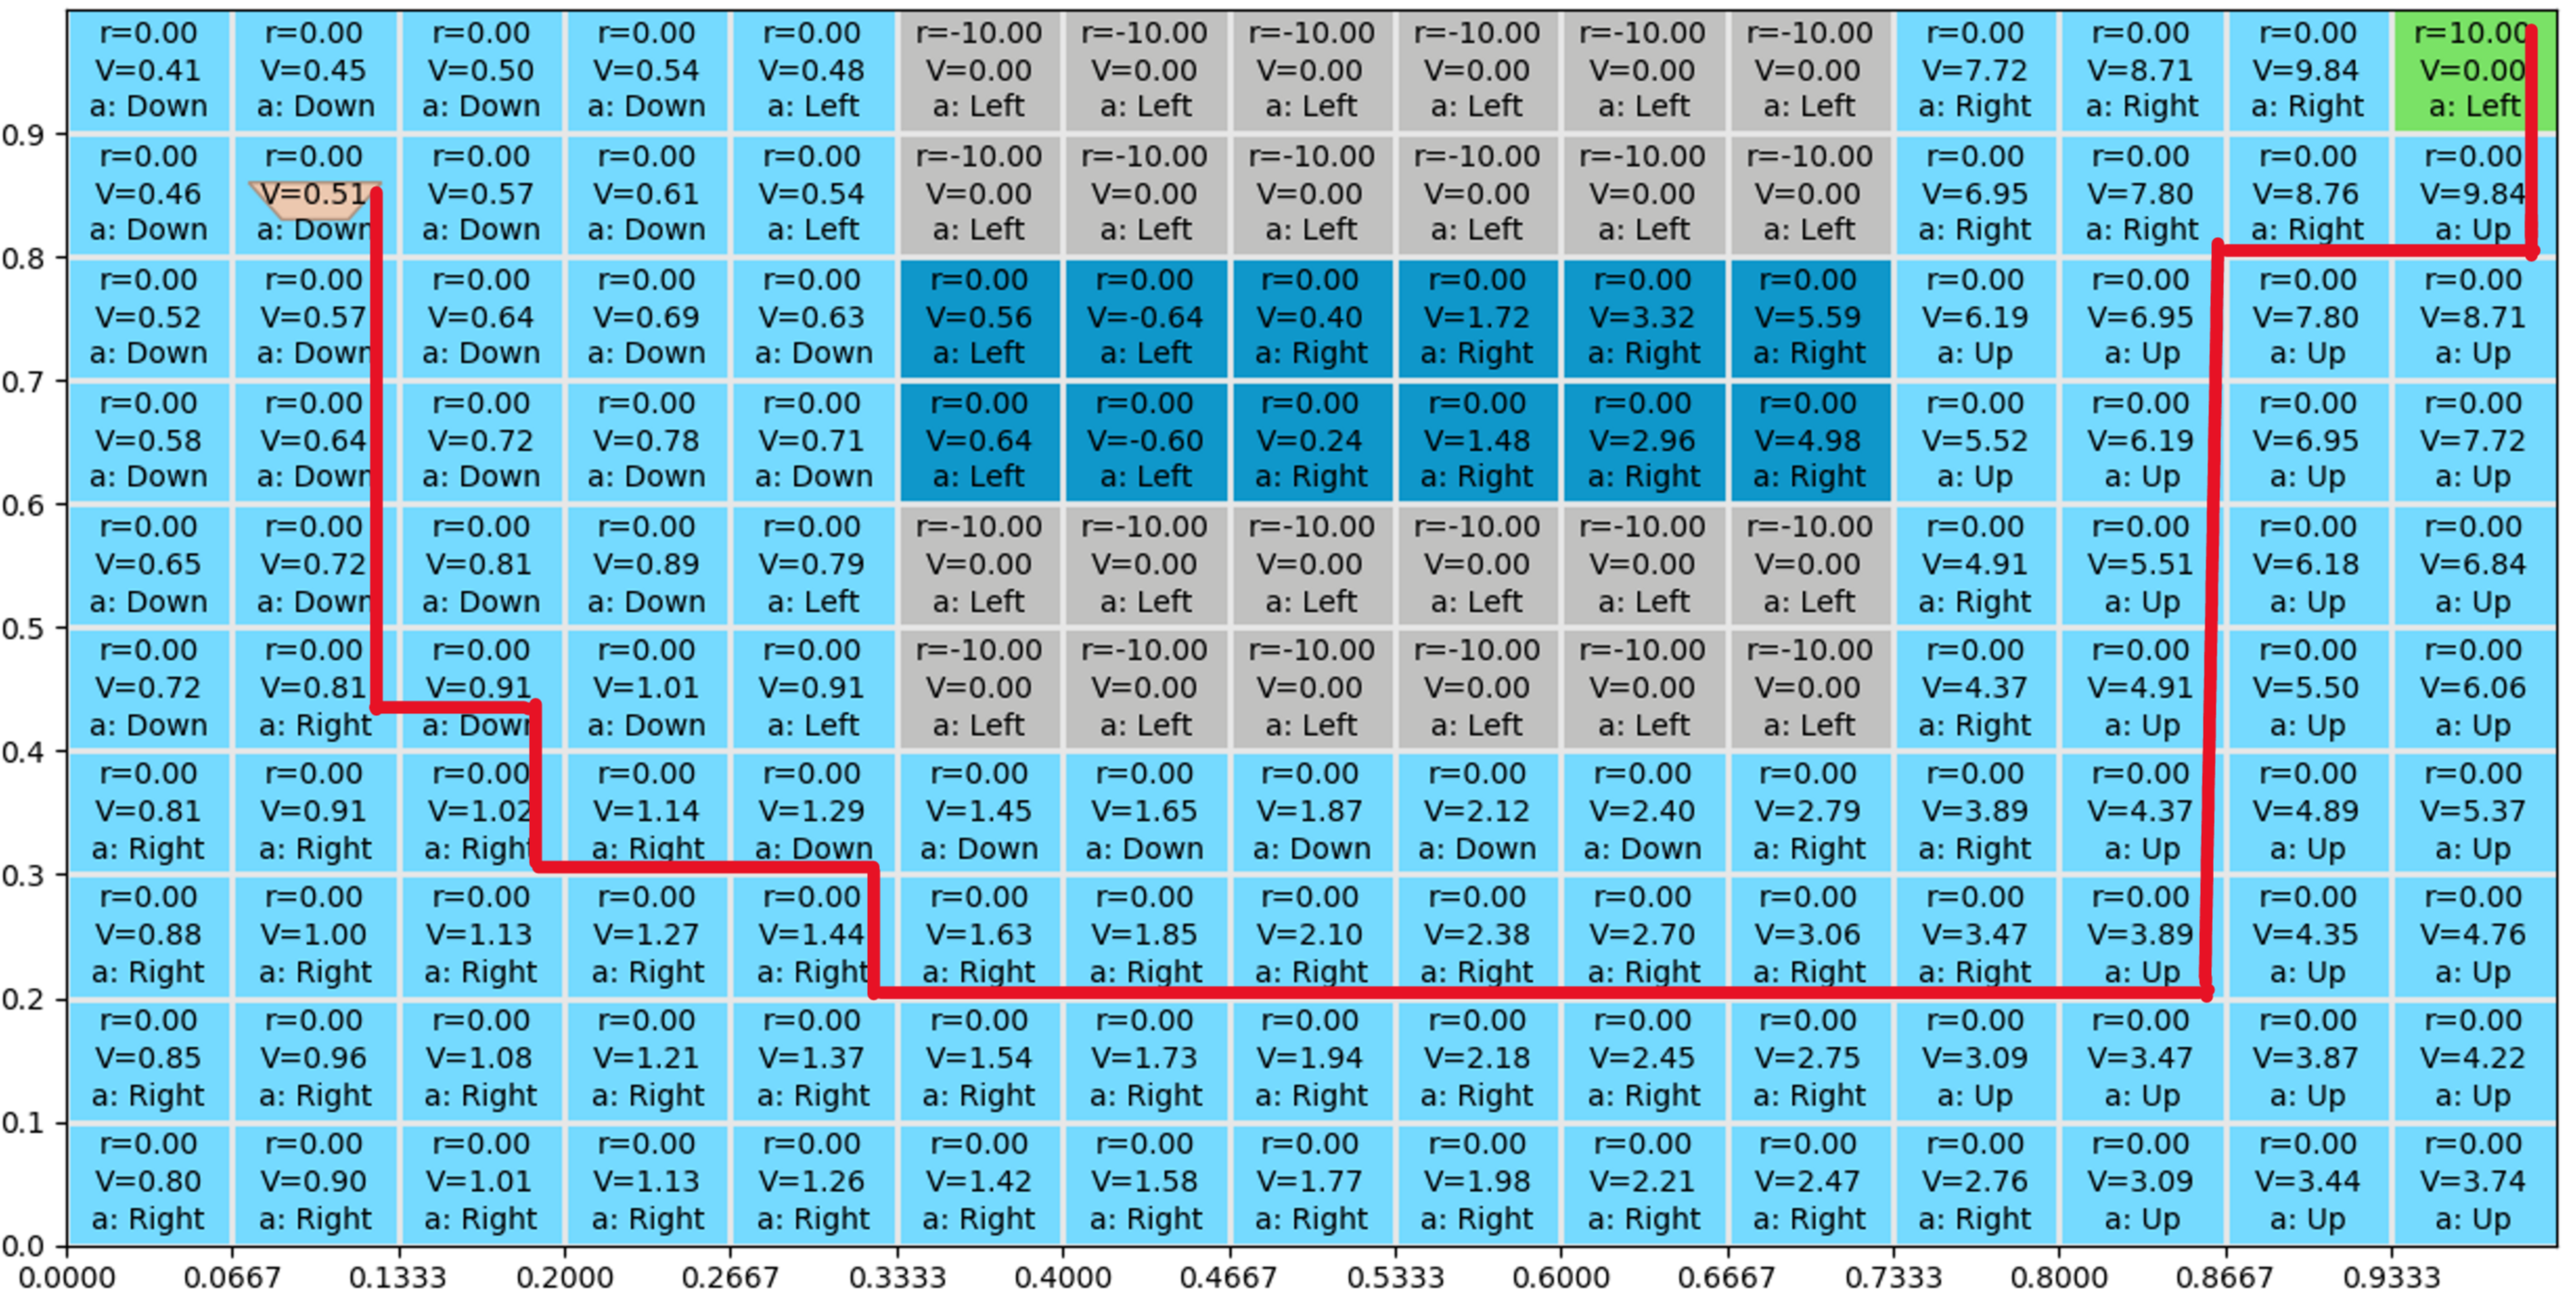
\includegraphics[width=\textwidth]{Paranoid_Sailor_path.png}
    \caption{State Values and Most probable path for \textit{paranoid} sailor}
    \label{fig-paranoid-sailor-path}
\end{figure}
\clearpage
\section{Question 4}
The algorithm does to converge with fewer than 100 iterations. The value function and policy still converge to the optimal in 30 or so iterations. As the policy of the agent depends on the state values, there seems to be no lag in the convergence. Hence both policy and value function converge at the same rate.
\section{Question 5}
The discounted returns for the starting state of $(1,8)$ are as follows 
\begin{itemize}
    \item $\mu_{G} = 0.6344$
    \item $\sigma_{G} = 1.345$
\end{itemize}
We see that the discounted reward is similar to the value function of the state. The reason is that the value function is just the expected value of a given state $s$ the discounted reward given that the agent starts from the state $s$. 
\[
v_{\pi}(s) \doteq \mathbb{E}_{\pi} \left [ G_{t} | S_{t}=s \right ]
\]
Hence the value function of a state is equal to the mean of the discounted rewards.
\section{Question 6}
No the value iteration approach cannot be applied to the suggested problem. Value iteration converges under the conditions that we have complete knowledge of the state space and to some degree know the dynamics of the system. In the given problem when the robot is navigating an unknown environment the assumptions of this knowledge of the state space, rewards, and transition probabilities are unrealistic.
\end{document}